
\documentclass[a4paper,10pt]{letter}


\usepackage[USenglish]{babel} %francais, polish, spanish, ...
\usepackage[T1]{fontenc}
\usepackage[ansinew]{inputenc}

\usepackage{lmodern} %Type1-font for non-english texts and characters

\usepackage{graphicx} %% Images can be included using \includegraphics{Dateiname}

\address{\textbf{Team B}\\
BUTEAU Paul-\'Emile\\
WISSOCQ Julien}

\signature{BUTEAU \& WISSOCQ}

%\date{\today} %%If commented, the current date is used in a short form
%\labelstyle{plain} %%Type of Labels: only plain is possible
%\makelabels %%Generates Labels
%\pagestyle{empty}

\begin{document}

\begin{letter}{\textbf{Client}\\ 
               IMAI Junichi\\}

\opening{\vspace{50pt}
\textbf{Recommendation for financial product}}

Dear client,

You asked us to give our conclusion about the knock-in 60\% sold by Daiwa Securities Group Inc. You can find a detailed analysis in the supplementary notes we joined for you.

Let us start first with the rating of the product: A by Standard\&Poors and A2 by Moody's.
Thus the two well-known financial institutions agreed to say that the product is judged quite risky. It features a cumulative default rate of 0.34\% over the 3 years of the maturity, compared with a quasi-0\% you can find for a AAA-product rated by S\&P.

Plus, you take some risk for an investment return of only 3\% per year. Either you want to minimize the risk by hedging your portfolio, then the interest rate is not a big issue, or you focus on this interest rate that you want to maximize, then you accept the risk. But choosing an intermediate product such as the one sold by Daiwa is not a good option. Whatever is your priority between risk-free capital or high return, the product will not fit your strategy.

Going deeper, the main result of our code shows that you will have 40\% of probability to earn money, thus 60\% to lose money. This is somewhat a bad start. Unfortunately, the potential gains are quite low: you can hope to a maximum of 9\% of return on investment over 3 years without interruption of the product. But concerning the loss, that is to mean that at least one index price among both will fall under 60\% of its initial value, and the index price will have trouble reaching its initial value: your loss will already be worth 40\%. That explains why we find a average gain that is negative (of course because Daiwa Co. will take a margin on his product) but very negative: about -26\%. Most surprisingly, the standard deviation of the gain is also low, about 8\%. Summing it up, if you invest 10 million of yen in this product, we estimate that you will lose 2.6 million yen on average.

Finally we should think about what will happen next in the real world, by simply looking at the evolution graphs of the two index prices that we consider: S\&P500 and Nikkei225. (You can find them in the detailed analysis attached.) We can see that over 10 years of data, the Nikkei225 value is average, but the S\&P500 is higher than never. Daiwa make a bet that this second index value will decrease at least by 60\% of its current value: and it is largely feasible. We should keep in mind that the value before 2005 was about 1200, and now it is about 2000. If they won this bet, you will no longer be covered, and you will have already a loss of 40\% of your investment.

Plus our model did not take into account any risk of future major financial crisis as the one we underwent in 2008, and indeed the model concerning crisis are barely reliable. But in today's unstable world, investors should be very watchful of such unpredictable events.

%\centering
%\caption{Evolution of S\&P (left) and Nikkei (right) over 10 years}
%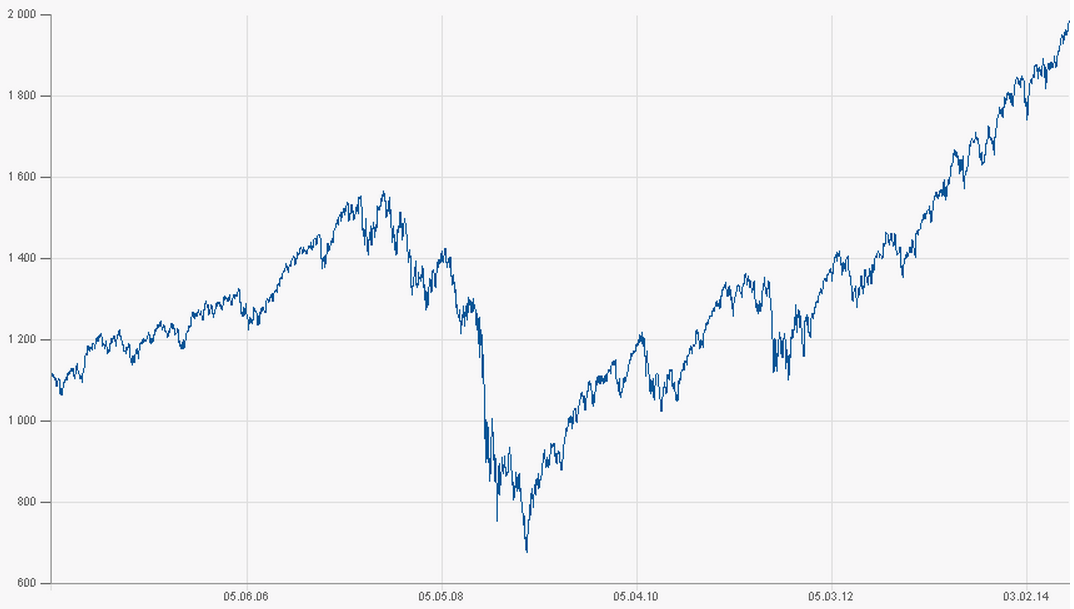
\includegraphics[width=\textwidth]{../SandP500_evolution}
%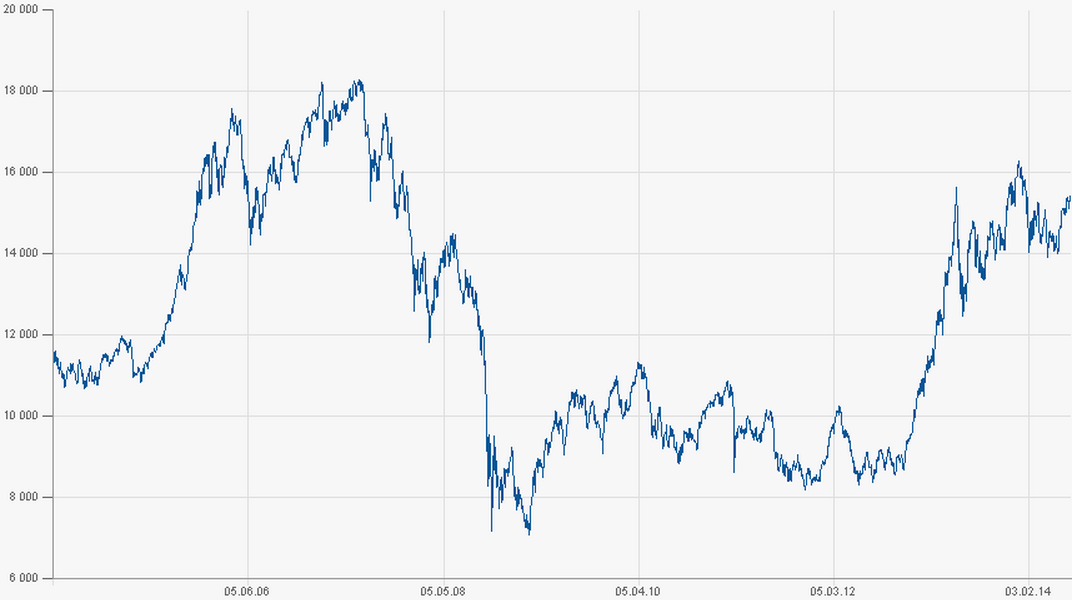
\includegraphics[width=\textwidth]{../Nikkei225_evolution}

That is why we think that this product as it was made is quite dangerous for any investment.

\closing{Sincerely, yours}

%\ps{PostScriptum. Whatever you forgot to say before.} %%PostScriptum

%\encl[Enclosings]{Text about enclosings} %%Enclosings

\end{letter}




\end{document}
